\card{Schnittstellen und Verträge}{
	\begin{enumerate}
		\item Schnittstellen müssen spezifiziert sein, manchmal können andere Objekte parallel entwickelt werden
		\item unterschiedliche Schnittstellen pro Objekt/Modul möglich
		\item benutzen von UML Klassendiagrammen
		\item Operationen A, B gleichzeitig, if \dots A \dots B \dots and \dots B \dots A \dots ist möglich (logische Parallelisierung, Ausführung auf verschiedener \\Hardware, A/B nicht Datenfluss-unabhängig
		\item benutzen von vererbter Parallelisierung zur Verteilung des Systems
		\item benutzen eines Aktivitätendiagramms zur Modellierung von Arbeitsflüssen, wie Workflows, dicke Barren sind Synchronisationspunkte, "`Swim-Lanes"' sind Abtrennungen, die verschiedene Systeme bezeichnen
	\end{enumerate}
}

\card{Design-by-Contract (Eiffel-Sprache)}{
	\begin{enumerate}
		\item Server muss die \textit{Postcondition} gewährleisten, kann die \textit{Precondition} annehmen
		\item Client muss die \textit{Precondition} gewährleisten, kann die \textit{Postcondition} annehmen
		\item UML Object Constraints Language (OCL):\\
			\begin{minipage}{0.35\textwidth}
				\scalebox{0.55}{\input{pictures/hashtable.pgf}}
			\end{minipage}\hfill
			\begin{minipage}{0.65\textwidth}
				\begin{description}
				\item[put:]precondition: !containsKey(key), \\postcondition: get(key==entry)
				\item[get:]precondition: containsKey(key), \\postcondition: !containsKey(key))
				\item[remove:]precondition: containsKey(key), \\postcondition:\\!containinsKey(key)
				\end{description}
			\end{minipage}
	\end{enumerate}
}

\card{Subcontracts (Vererbung)}{
	möglicherweise Subkonstruktor
	\begin{enumerate}
		\item beibehalten oder schwächen der Precondition (mehr kann reinkommen)
		\item beibehalten oder stärken der Postcondition (weniger kann heraus)
	\end{enumerate}
	\hspace*{1cm}\scalebox{0.5}[0.5]{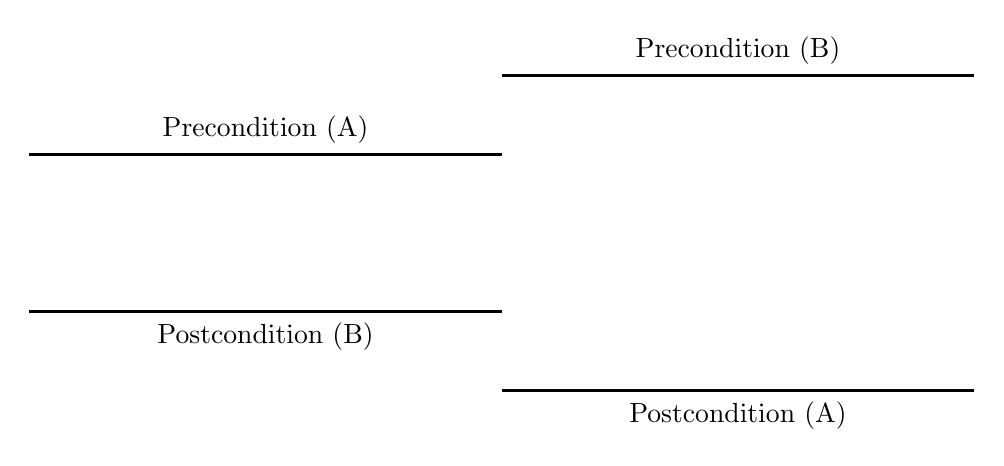
\begin{tikzpicture}[]
\draw[very thick] (0,1)to node[below] {Postcondition (B)}(6,1);
\draw[very thick] (0,3)to node[above] {Precondition (A)}(6,3);

\draw[very thick] (6,0)to node[below] {Postcondition (A)}(12,0);
\draw[very thick] (6,4)to node[above] {Precondition (B)}(12,4);
\end{tikzpicture}}
}

\card{Data Dictonaries}{
	\begin{enumerate}
		\item low-level Datenentscheidungen (spät im Designprozess)
		\item Repräsentation von Datenstrukturen (nur für diejenigen bekannt mit direkten Dateninteraktionen (Information hiding))
		\item Liste von allen Namen, Einheiten, Beziehungen, benutzten Attributen (Namenmanagement, Vermeidung von Duplikaten, Wissen über Speicherorganisation)
	\end{enumerate}
}